\section{Regularization} \label{sec:regularization}

When dealing with many candidates to use as covariates, one has to deal with the problem of selecting a subset of variables to use in constructing the model. 
This means that the vector of coefficients $\beta_j = [ \beta_{1 j} \cdots \beta_{pj} ]$ should not have all nonzero values.
There are many ways of selecting a subset of variables among the available options.
Classical approaches for this problem are the Stepwise algorithm \cite{efroymson1960multiple}, \cite{hocking_selection_1967}, \cite{tibshirani1996regression}, which includes variables in sequence. 

Two approaches will be employed. At first, we use a Mixed Integer Linear Programming optimization problem (MILP) to find the best subset among all choices of covariates. The second way is by using a LASSO-type technique, which consists in penalizing the $\ell_1$-norm of regressors, thus shrinking the size of estimated coefficients towards zero.  

\subsection{Best subset selection via MILP}
\label{sec:best-subset-mip}

We use MILP to select variables by including constraints which limits their number in $K$. Only $K$ coefficients $\beta_{pj}$ may have nonzero values, for each $\alpha$. 
Binary variable $z_{pj}$ indicates whether $\beta_{pj}$ has a nonzero value. 
The optimization problem that incorporates this idea is described below:
\begin{IEEEeqnarray}{lr}
 \underset{\beta_{0j},\beta_j,z_{p j} \varepsilon_{t j}^{+},\varepsilon_{t j}^{-}}{\text{min}} \sum_{j \in J} \sum_{t\in T}\left(\alpha_j\varepsilon_{t j}^{+}+(1-\alpha_j)\varepsilon_{t j}^{-}\right)  \span \label{eq:mip0}  \\
\mbox{subject to} \span \nonumber \\
\varepsilon_{t j}^{+}-\varepsilon_{t j}^{-}=y_{t}-\beta_{0 j}- \beta_{j}^T x_{t}, \span \nonumber  \\
& \forall t \in T ,\forall j \in J, \label{eq:mip1}  \\
\varepsilon_{t j}^{+},\varepsilon_{t j}^{-}\geq0,&\forall t \in T ,\forall j \in J, \label{eq:mip2}\\
- M z_{p j} \leq \beta_{p j} \leq M z_{p j},& \forall j \in J, \forall p\in P, \label{eq:mip3}\\
\sum_{p \in P} z_{p j} \leq K, &  \forall j \in J, \label{eq:mip4}\\
z_{p j} \in \{0,1\}, & \forall j \in J,  \forall p\in P, \label{eq:mip5}\\
\beta_{0j} + \beta_{j}^T x_{t} \leq \beta_{0,j+1} + \beta_{j+1}^T x_{t},  \nonumber \\
& \forall t \in T, \forall j \in J_{(-1)}, \label{eq:mip6}
\end{IEEEeqnarray}
%\begin{flalign}
%\underset{\beta_{0\alpha},\beta_\alpha,z_{p \alpha}, \varepsilon_{t j}^{+},\varepsilon_{t j}^{-}}{\text{min}} \sum_{j \in J} \sum_{t\in T}\left(\alpha\varepsilon_{t j}^{+}+(1-\alpha)\varepsilon_{tj}^{-}\right) \span \span \label{eq:mip0}   \\
%\mbox{s.t } \nonumber \\
%& \varepsilon_{t j}^{+}-\varepsilon_{t j}^{-}=y_{t}-\beta_{0 \alpha}-\sum_{p \in P}\beta_{p j}x_{t,p}, \span  \label{eq:mip1} \\
%& &  \forall t \in T ,\forall j \in J,  \nonumber\\
%& \varepsilon_{t j}^{+},\varepsilon_{t j}^{-}\geq0, & \forall t \in T ,\forall j \in J, \label{eq:mip2}\\
%& - M z_{p \alpha} \leq \beta_{p j} \leq M z_{p \alpha},& \forall j \in J, \forall p\in P, \label{eq:mip3}\\
%& \sum_{p \in P} z_{p \alpha} \leq K, & \forall j \in J, \label{eq:mip4}\\
%& z_{p \alpha} \in \{0,1\}, & \forall j \in J,  \forall p\in P, \label{eq:mip5}\\
%& \beta_{0\alpha} + \beta_{\alpha}^T x_{t} \leq \beta_{0\alpha'} + \beta_{\alpha'}^T x_{t}, \span \label{eq:mip6} \\
%& & \forall t \in T, \forall (\alpha, \alpha') \in A \times A,  \alpha < \alpha',   \nonumber
%\end{flalign}
The objective function and constraints (\ref{eq:mip1}), (\ref{eq:mip2}) and (\ref{eq:mip6}) are the same from standard linear quantile regression. 
By constraint (\ref{eq:mip3}), variable $z_{p j}$ is a binary that assumes 1 when coefficient $\beta_{p j}$ is included, while (\ref{eq:mip4}) guarantees that at most $K$ of them are nonzero.
The value of $M$ is chosen in order to guarantee that $M \geq \|\hat{\beta_hj}\|_{\infty}$. The solution given by $\beta_{0j}^*$ and $\beta_j^* = [ \beta_{1 j}^* \cdots \beta_{pj}^* ]$ will be the best linear $\alpha$-quantile regression with $K$ nonzero coefficients.  

\subsubsection{Defining groups for variables}

Consider the optimization problem defined on (\ref{eq:mip0})-(\ref{eq:mip6}). The choice of the best subset is independent for different values of probabilities $\alpha$. This means that the best subset may include two completely different sets of regressors for two probabilities $\alpha_j$ and $\alpha_{j+1}$. Take $K=2$ for the example, selecting $\beta_{1j}$ and $\beta_{4j}$ for $j$ while $\beta_{2,j+1}$ and $\beta_{5,j+1}$ is possible, but unlikely to be true.  

To address this issue, we propose to divide all $j \in J$ in groups. The collection $G$ of all groups $g$ form a partition of $A$, and each $\alpha$ belongs to exactly one group $g$. 
The subset of selected covariates must be the same for all $j$ in the same group $g$. To model these properties as constraints on problem (\ref{eq:mip0})-(\ref{eq:mip6}), we substitute constraint (\ref{eq:mip3}) for the following equations:
\begin{IEEEeqnarray}{lr}
z_{p j g} := 2 - ( 1-z_{pg}) - I_{gj}\span  \label{mipgrupzpa} \\
\sum\limits_{g \in G} I_{gj} = 1, &\forall j \in J,\label{eq:mipgrupa} \\
-Mz_{p j g}  \leq  \beta_{p j} \leq M z_{p j g}, \nonumber \\ 
& \forall p \in P, \forall j \in J,  \forall g \in G,  \label{eq:mipgrupb} \\
I_{gj}, z_{pg} \in \{0,1\}, & \forall p \in P,  \forall g \in G, \label{eq:mipgrupc}
\end{IEEEeqnarray}
%\begin{align} - DUAS COLUNAS
%z_{p \alpha g} := 2 - ( 1-z_{pg}) - I_{g\alpha}\span \span \label{mipgrupzpa} \\
%\sum\limits_{g \in G} I_{g\alpha} = 1, & \forall j \in J,\label{eq:mipgrupa}& \\
%-Mz_{p \alpha g}  \leq  \beta_{p \alpha g} \leq M z_{p \alpha g}, \forall p \in P, \forall j \in J,  \forall g \in G, \span \span \label{eq:mipgrupb} \\
%&I_{g\alpha}, z_{pg} \in \{0,1\},& \, \forall p \in P,  \forall g \in G, \label{eq:mipgrupc}
%\end{align}
on problem (\ref{eq:mip0})-(\ref{eq:mip6}).
where $G$ is a set of group index and $z_{pg}$ is a binary variable that equals 1 iff covariate $p$ is included on group $g$ and $I_{gj}$ equals 1 iff the $j$\textsuperscript{th} quantile belongs to group $g$. 
Constraint (\ref{eq:mipgrupb}) forces that 
$$\text{if }z_{pg} = 0 \text{ and }I_{gj} =1 \text{ then } \beta_{p j = 0}.$$
Hence, if covariate $p$ belongs to group $g$, this covariate is not among group's $g$ subset of variables, than its coefficient must be equal to $0$, for that $j$.
Note that variable $z_{p j}$ behaves differently than when we are not considering groups. This means that if the $j$\textsuperscript{th} quantile belongs to group $g$ but variable $p$ is not selected to be among the ones of group $g$, than $\beta_{pj}$ is zero.
Equation (\ref{mipgrupzpa}) defines $z_{pj}$ to simplify writing. 


%\subsubsection*{Defining groups for variables where each group consists of probabilities in sequence}
%%
%Each groups $g \in G$, as defined on the last section, may be any combination of probabilities $\alpha$, such that they don't be in sequence. Figure \ref{fig:heatmap-exemplo-grupos} shows an example of 
%
%\begin{figure}
%	\centering
%	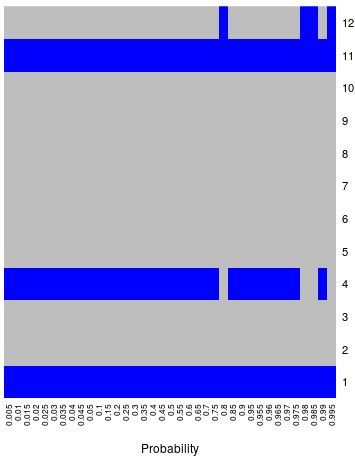
\includegraphics[width=0.4\linewidth]{Figuras/betas-mip/heatmap-exemplo-grupos}
%	\caption{}
%	\label{fig:heatmap-exemplo-grupos}
%\end{figure}
%
%
%\begin{eqnarray}
%\underset{\beta_{0\alpha},\beta_\alpha,z_{p \alpha}, \phi_{p \alpha}, \varepsilon_{t j}^{+},\varepsilon_{t j}^{-}}{\text{min}} & \sum_{j \in J} \sum_{t\in T}\left(\alpha\varepsilon_{t j}^{+}+(1-\alpha)\varepsilon_{tj}^{-}\right) \label{eq:mipgr0} \\
%\mbox{s.t } & \varepsilon_{t j}^{+}-\varepsilon_{t j}^{-}=y_{t}-\beta_{0 \alpha}-\sum_{p \in P}\beta_{p j}x_{t,p},& \qquad\forall t \in T ,\forall j \in J, \label{eq:mipgr1}\\
%& \varepsilon_{t j}^{+},\varepsilon_{t j}^{-}\geq0,&\qquad\forall t \in T ,\forall j \in J, \label{eq:mipgr2}\\
%& - M z_{p \alpha} \leq \beta_{p j} \leq M z_{p \alpha},&\qquad \forall j \in J, \forall p\in\{1,\dots,P\}, \label{eq:mipgr3}\\
%& \sum_{p \in P} z_{p \alpha} \leq K, & \qquad \forall j \in J, \label{eq:mipgr4}\\
%& z_{p \alpha} \in \{0,1\},&\qquad \forall j \in J, \forall p\in\{1,\dots,P\}, \label{eq:mipgr5}\\
%& \beta_{0\alpha} + \beta_{\alpha}^T x_{t} \leq \beta_{0\alpha'} + \beta_{\alpha'}^T x_{t}, & \qquad \forall t \in T, \forall (\alpha, \alpha') \in A \times A,  \alpha < \alpha',\nonumber\\ \label{eq:mipgr6} \\
%& z_{p\alpha} - z_{p\alpha+1} \leq m_{p\alpha}, & \qquad \forall j \in J', \qquad \forall p \in P  \\
%& \sum_{j \in J'} r_\alpha \leq |G| - 1 
%\label{eq:mipgr} \\
%\end{eqnarray}
%where $A' = A\setminus \{|A|\}$

\subsubsection{Inclusion of derivative penalty}
Our estimation procedure consists of a different model for each $\alpha$-quantile. From the assumption that the value of similar quantiles be produced by similar models, we need to prevent big changes on the $p$ coefficient $\beta_p(\alpha)$ when seen as a function of probability $\alpha$, as shown on Figure \todoi{adicionar figura}. On the implementation side, we must limit the second difference of the sequence of coefficients $\{\beta_{pj}\}_{j \in J}$ for every parameter $p$. This will bring smoothness to $\beta_p(\alpha)$.

for a parameter $p$, must have limited second difference, bringing smoothness to the change of coefficients. By including this constraint, every time a variable enters or leaves the subset, its values must be increasing or decreasing smoothly. The second order differential of coefficients is given by the equation below:
\begin{equation}
\tilde{D}_{pj}^{2}:=\frac{\left(\frac{\beta_{p,j+1}-\beta_{pj}}{\alpha_{j+1}-\alpha_{j}}\right)-\left(\frac{\beta_{p,j}-\beta_{p,j-1}}{\alpha_{j}-\alpha_{j-1}}\right)}{\alpha_{j+1}-2\alpha_{j}+\alpha_{j-1}}.
\end{equation}
This idea is implemented on the optimization problem by adding a penalty on the objective function to penalize the absolute value $|D_{pj'}^{2}|$ by a tuning parameter $\gamma$, that controls how rough the sequence $\{\beta_{pj}\}_{j \in J}$ can be. The full optimization problem for the best subset selection via MILP which incorporates the derivative penalty is given below:
\begin{IEEEeqnarray}{lr}
	\underset{\beta_{0j},\beta_j,z_{p j} \varepsilon_{t j}^{+},\varepsilon_{t j}^{-}}{\text{min}} \sum_{j \in J} \sum_{t\in T}\left(\alpha_j\varepsilon_{t j}^{+}+(1-\alpha_j)\varepsilon_{tj}^{-}\right) \nonumber \span \\
	& + \gamma \sum_{j \in J'} D2_{pj}   \\
	\mbox{subject to} \span \nonumber \\
	\varepsilon_{t j}^{+}-\varepsilon_{t j}^{-}=y_{t}-\beta_{0 j}-\beta_{j}^T x_{t,p},& \forall t \in T ,\forall j \in J,\\
	\varepsilon_{t j}^{+},\varepsilon_{t j}^{-}\geq0, & \forall t \in T ,\forall j \in J, \\
	- M z_{p \alpha} \leq \beta_{p j} \leq M z_{p \alpha}, & \forall j \in J, \forall p\in P, \\
	\sum_{p \in P} z_{p \alpha} \leq K, & \forall j \in J, \\
	z_{p \alpha} \in \{0,1\}, & \forall j \in J,  \forall p\in P, \\
	D2_{pj} >  \tilde D_{pj}^{2} &  \forall j \in J_{(-1)}, \forall p\in P, \\
	D2_{pj} > - \tilde D_{pj}^{2} &  \forall j \in J_{(-1)}, \forall p\in P,\\
\beta_{0j} + \beta_{j}^T x_{t} \leq \beta_{0,j+1} + \beta_{j+1}^T x_{t},&\forall t \in T, \forall j \in J_{(-1)}, 
\end{IEEEeqnarray}
where $A'$ is the set formed by the same elements of $A$ without the first and the last elements.

\subsection{Variable selection via LASSO}
\label{sec:best-subset-ell1}

Another way of doing regularization is including the $\ell_1$-norm of the coefficients on the objective function. In \cite{belloni_l1-penalized_2009}, the reader can find properties and convergence rate when using the LASSO to select variables in a quantile regression setting. The ADALASSO variant is presented in \cite{ciuperca_adaptive_2016}. 
The advantage of this method is that coefficients are shrunk towards zero by changing a continuous parameter $\lambda$, which penalizes the size of the $\ell_1$-norm.  
When the value of $\lambda$ gets bigger, fewer variables are selected to be used. 
This is the same strategy of the LASSO methodology, and its usage for the quantile regression is discussed in \cite{li2012l1}.
On the litterature, the LASSO QR regularization is applied for only a single quantile by the following optimization problem:
\begin{equation}
\underset{\beta_{0\alpha},\beta_\alpha}{\text{min}} \sum_{t \in T}\alpha|y_{t}-q_\alpha(x_t)|^{+}+ \sum_{t \in T}(1-\alpha)|y_{t}-q_\alpha(x_t)|^{-}+\lambda\|\beta_\alpha\|_{1},
\label{eq:l1-qar-optim}
\end{equation}
\[
q_\alpha(x_t)=\beta_{0}-\beta^T x_{t}.
\]
In our problem, however, we need to estimate multiple quantiles in a way that the issue of crossing quantiles is circumvented. So, we use for the LASSO the same formulation of estimating all quantiles simultaneously with a non crossing constraint relating each quantile function.



The process of estimation is done in two stages: variable selection and coefficients estimation. At first, all normalized covariates\footnote{For such estimation to be coherent each covariate must have the same relative weight in comparison with one another, i.e., they must be normalized. 
This normalization process is a linear transformation to each covariate such that all have mean $\mu = 0$ and variance $\sigma^2 = 1$. 
We apply the transformation $\tilde{x}_{t,p} = (x_{t,p} - \bar{x}_{t,p}) / \hat\sigma_{x_{t,p}}$, where $\bar{x}_{t,p}$ and $\hat{\sigma}_{x_{t,p}}$ are respectively the sample's unconditional mean and standard deviation. The $\tilde{y}_{t-p,i}$ series will be used to estimate the coefficients, as this series has the desired properties.} are input on the following optimization problem:
\begin{IEEEeqnarray}{lr}
\tilde \beta_\lambda^{*LASSO} = \underset{\beta_{0},\beta,\varepsilon_{t j}^{+},\varepsilon_{t j}^{-}}{\text{arg min}} \sum_{j \in J} \sum_{t \in T}(\alpha_j\varepsilon_{t j}^{+}+(1-\alpha_j)\varepsilon_{t j}^{-}) \span \nonumber \\
\hspace{3.5cm} +\lambda\sum_{p \in P}\mbox{\ensuremath{\xi}}_{p j} + \gamma \sum_{j \in J'} D2_{pj} \span \label{eq:obj-lasso} \\
\mbox{subject to } \nonumber & \\
\varepsilon_{t j}^{+}-\varepsilon_{t j}^{-}=y_{t}-\beta_{0 j}-\beta_{j}^T x_{t,p},& \forall t \in T ,\forall j \in J,\\\varepsilon_{t j}^{+},\varepsilon_{t j}^{-}\geq0,&\forall t \in T, \forall j \in J,\\
\xi_{pj}\geq\beta_{p j},&\forall p\in P, \forall j \in J,  \label{l1-qar-3}
\\
\xi_{pj}\geq - \beta_{p j},&\forall p\in P, \forall j \in J,  \label{l1-qar-4}
\\
	D2_{pj} >  \tilde D_{pj}^{2} &  \forall j \in J_{(-1)}, \forall p\in P, \\
D2_{pj} > - \tilde D_{pj}^{2} &  \forall j \in J_{(-1)}, \forall p\in P,\\
\beta_{0j} + \beta_{j}^T x_{t} \leq \beta_{0,j+1} + \beta_{j+1}^T x_{t},&\forall t \in T, \forall j \in J_{(-1)}, \label{eq:l1-qar5}
\end{IEEEeqnarray}
This model is built upon the standard linear programming model for the quantile regression (\ref{eq:linear-opt-1})-(\ref{eq:linear-opt-ult}). 
On the above formulation, the $\ell_1$ norm of equation (\ref{eq:l1-qar-optim}) is substituted by the sum of $\xi_p$, which represents the absolute value of $\beta_{pj}$. The link between variables $\xi_p$ and $\beta_{pj}$ is made by constraints (\ref{l1-qar-3}) and (\ref{l1-qar-4}). Note that the linear coefficient $\beta_{0j}$ is not included in the penalization, as the sum of penalties on the objective function \ref{eq:obj-lasso}.

% % % % % % % % Esse trecho deve ser usado quando os coeficientes do lasso forem utilizados, e não apenas o lasso sendo um seletor de variáveis % % % % % % % % %
%Each component of the output $\tilde \beta_\lambda^{*LASSO}$ must be corrected by multiplying each coefficient for its standard deviation: $\beta_{p\alpha,\lambda}^{*LASSO} = \tilde \beta_{p\alpha,\lambda}^{*LASSO} \hat\sigma_{x_{t,p}}$.
%\begin{eqnarray}
%\tilde \beta_\lambda^{*LASSO} = \underset{\beta_{0},\beta,\varepsilon_{t j}^{+},\varepsilon_{t j}^{-}}{\text{arg min}} & \sum_{j \in J} \sum_{t \in T}\left(\alpha\varepsilon_{t j}^{+}+(1-\alpha)\varepsilon_{t j}^{-}\right)+\lambda\sum_{p \in P}\mbox{\ensuremath{\xi}}_{p \alpha} \label{eq:obj-lasso} \\
%\mbox{subject to } & \varepsilon_{t j}^{+}-\varepsilon_{t j}^{-}= y_{t}-\beta_{0 \alpha}-\sum_{p \in P}\beta_{p j}\tilde x_{t,p},&\forall t\in T, \forall j \in J, \\
%& \varepsilon_{t j}^{+},\varepsilon_{t j}^{-}\geq0,&\forall t \in T, \forall j \in J,\\
%& \xi_{pj}\geq\beta_{p j},&\forall p\in P, \forall j \in J,  \label{l1-qar-3}
%\\
%& \xi_{pj}\geq-\beta_{p j},&\forall p\in P, \forall j \in J.  \label{l1-qar-4}
%\end{eqnarray}

For low values of $\lambda$, the penalty over the size of coefficients is small. Because of that, the output of problem (\ref{eq:obj-lasso})-(\ref{l1-qar-4}) is a model where most coefficients have nonzero value. On the other hand, when the penalty on $\| \beta_j \|_1$ is big, many covariates will have zero valued coefficients. When $\lambda$ approaches infinity, one has a constant model. 
For instance, the penalty isn't applied to the linear coefficient $\beta_{0j}$. 

In fact, the LASSO coefficients are biased, so it is employed only as a variable selector. 
The optimum vector of coefficients $\tilde \beta_\lambda^{*LASSO}$ for a given $\lambda$ may be composed by both nonzero and zero coefficients. 
We then define $S_\lambda$ as the set of indexes of selected variables given by
\begin{equation*}
S_\lambda = \{ p \in \{ 1,\dots,P \} | \; |\beta^{*LASSO}_{\lambda,p}| \neq 0  \}.
\end{equation*}
Hence, we have that, for each $p \in \{ 1,\dots,P \}$,
$$\beta^{*LASSO}_{\lambda,p} = 0 \Longrightarrow \beta^{*}_{\lambda,p} = 0.$$

Note that problem (\ref{eq:linear-opt-1})-(\ref{eq:linear-opt-ult}) is employed to act as variable selection only. On the second stage, the optimal coefficient vector $\beta_\lambda^{*LASSO}$ is estimated by the non-regularized QR, where only variables that bellongs to $S_\lambda$ are input:
\begin{IEEEeqnarray*}{lr} (\mathcal{L}_{\lambda}^{*},\beta_{\lambda}^{*})\overset{(obj,var)}{\longleftarrow} \underset{\beta_{0j},\beta_j,z_{p j}, \varepsilon_{t j}^{+},\varepsilon_{t j}^{-}}{\text{min}} \sum_{j \in J} \sum_{t\in T}\left(\alpha_j \varepsilon_{t j}^{+}+(1-\alpha_j)\varepsilon_{t\alpha_j}^{-}\right) \span \nonumber
\\
&  + \gamma \sum_{j \in J'} D2_{pj} \\
\text{subject to } \span \nonumber \\
\varepsilon_{t j}^{+}-\varepsilon_{t j}^{-}=y_{t} - \beta_{0\alpha} - \sum_{p\in S_\lambda} \beta_p x_{t,p}, & \forall t \in T, \forall j \in J, \\
\varepsilon_{tj}^+,\varepsilon_{tj}^- \geq 0, &  \forall t \in T,\forall j \in J,\\ 
D2_{pj} >  \tilde D_{pj}^{2} &  \forall j \in J_{(-1)}, \forall p\in P, \\
D2_{pj} >  - \tilde D_{pj}^{2} &  \forall j \in J_{(-1)}, \forall p\in P,\\
\beta_{0j} + \beta_{j}^T x_{t} \leq \beta_{0,j+1} + \beta_{j+1}^T x_{t}, & \forall t \in T, \forall j \in J_{(-1)},
\end{IEEEeqnarray*}
The variable $\mathcal{L}_{\lambda}^{*}$ receives the value of the objective function on its optimal solution.
In summary, the optimization in equation \ref{eq:l1-qar-optim} acts as a variable selection for the subsequent estimation, which is normally called the post-LASSO estimation \cite{belloni2009least}.



% (\ref{eq:linear-opt-1})-(\ref{eq:linear-opt-ult}). 



